\section{Optimierungen des Bit-Array-Ansatzes}

\subsection{Bit-Array als Filter}

\begin{frame}
	\setbeamercolor{normal text}{fg=gray,bg=}
	\setbeamercolor{alerted text}{fg=black,bg=}
	\usebeamercolor{normal text}

	\begin{itemize}
		\setlength\itemsep{\stdItemSep}
		\item \alert<1->{Zwischenschritt:}
		\begin{itemize}
			\setlength\itemsep{\stdItemSep}
			\vspace*{\stdItemSep}
			\item \alert<1->{Obere Schranke des Jaccard-Index mit Bit-Arrays effizient bestimmen}
		\end{itemize}
		\item \alert<2->{Idee:}
		\begin{itemize}
			\setlength\itemsep{\stdItemSep}
			\vspace*{\stdItemSep}
			\item \alert<2->{$A$, $B$ - Mengen}
			\item \alert<3->{$A_{F}$ $=$ $bloom(A)$, $B_{F}$ $=$ $bloom(B)$ - Bit-Arrays der Mengen}
			\item \alert<4->{Es gilt:}
			\begin{itemize}
				\setlength\itemsep{\stdItemSep}
				\vspace*{\stdItemSep}
				\item \alert<4->{$|A_{F}|$ $\leq$ $|A|$}
				\item \alert<5->{$|A_{F} \vee B_{F}|$ $\leq$ $|A \cup B|$}
				\item \alert<6->{$jaccard(A, B)$ $=$ $\frac{|A \cap B|}{|A \cup B|}$} \alert<7->{$=$ $\frac{|A| + |B| - |A \cup B|}{|A \cup B|}$}
					\alert<8->{$\leq$ $\frac{|A| + |B| - |A_{F} \vee B_{F}|}{|A_{F} \vee B_{F}|}$}
			\end{itemize}
		\end{itemize}
		\item \alert<9->{Vorgehen:}
		\begin{itemize}
			\setlength\itemsep{\stdItemSep}
			\vspace*{\stdItemSep}
			\item \alert<9->{Schätze Jaccard-Index}
			\item \alert<10->{Größer Threshold? $\Rightarrow$ berechne Jaccard-Index}
		\end{itemize}
	\end{itemize}

	\uncover<9->
	{
		\begin{tikzpicture}[overlay]
			\node (start) at (2.5, 1.5) {};
			\node (end) at (8.7, 2.5) {};
			\path [draw, ->, green, very thick] (start) -- (end);
		\end{tikzpicture}
	}
	\uncover<10->
	{
		\begin{tikzpicture}[overlay]
			\node (start) at (5.5, 0.8) {};
			\node (end) at (6, 2.5) {};
			\path [draw, ->, blue, very thick] (start) -- (end);
		\end{tikzpicture}
	}
\end{frame}

\begin{frame}
	\vspace*{-.025cm}
	\hspace*{-.5cm}
	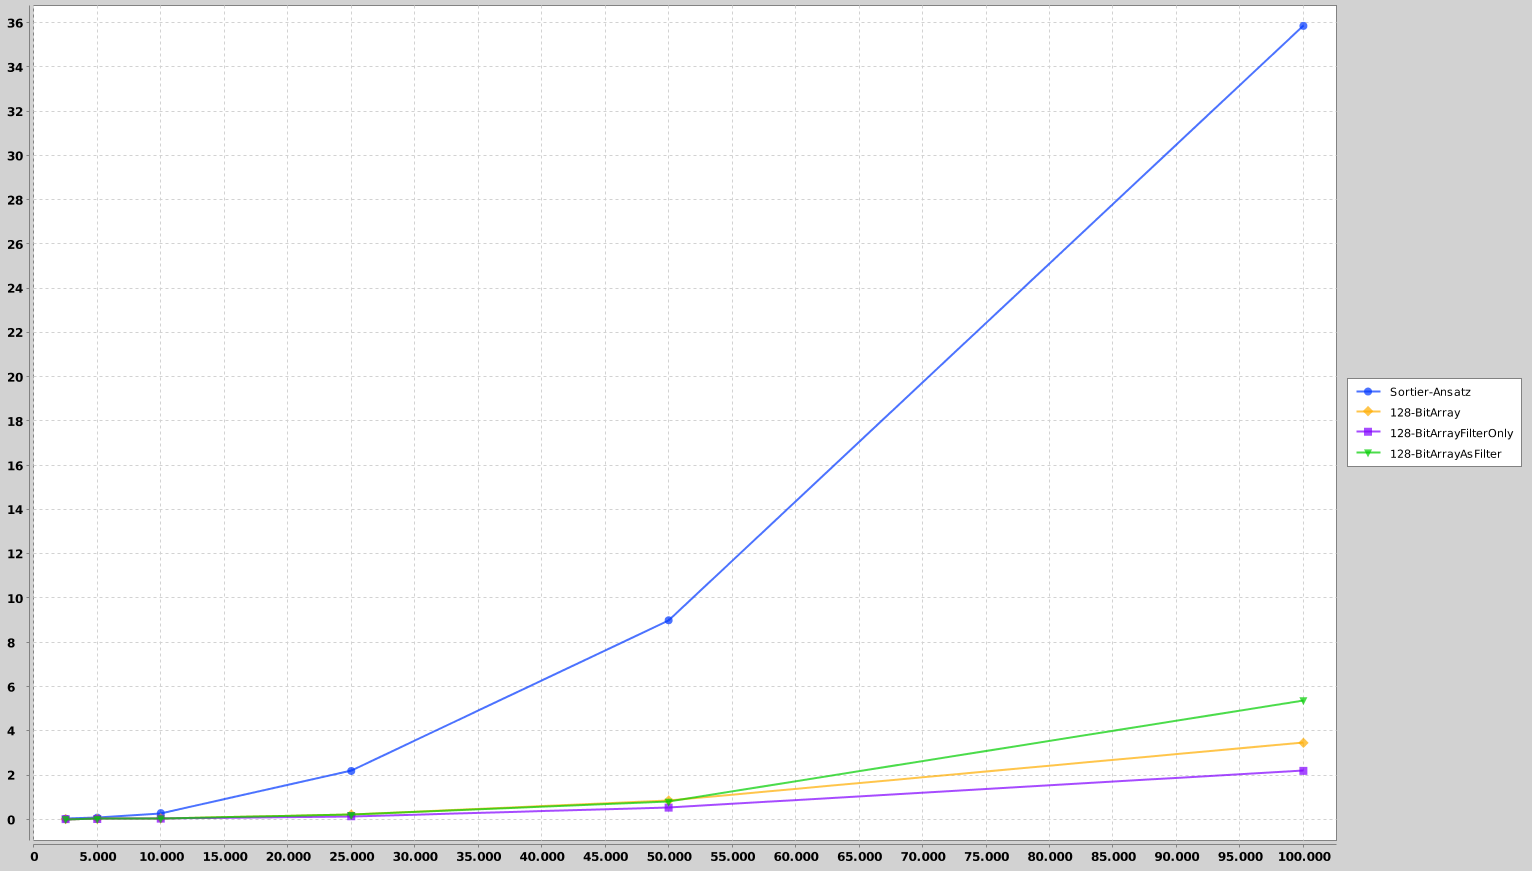
\includegraphics[width=1.07\textwidth, height=1.02\textheight]{Bilder/second_runtime_evaluation_for_threshold_0_7_trigram_one_fuzzy_date.png}

	\begin{tikzpicture}[overlay]
		\node at (3.6, 7)
		{
			\begin{footnotesize}
			\begin{varwidth}{0.6\textwidth}
			\textbf{Ausführungszeit in Minuten}
			\begin{itemize}
				\item für unterschiedlich große Datensätze
				\item Parameter
				\begin{itemize}
					\item Trigramme
					\item Threshold: $0.7$
					\item Datumsunschärfe: $1$
				\end{itemize}
				\item Testsystem
				\begin{itemize}
					\item CPU: 8 Kerne (HT) @ 3.4 GHz
					\item RAM: 16 GB
				\end{itemize}
			\end{itemize}
			\end{varwidth}
			\end{footnotesize}
		};
	\end{tikzpicture}

\end{frame}

\subsection{Filtern in 2 Phasen}

\begin{frame}
	\frametitle{Filtern in 2 Phasen}
	\begin{itemize}
		\setlength\itemsep{\stdItemSep}
		\item Phase 1
		\begin{itemize}
			\setlength\itemsep{\stdItemSep}
			\vspace*{\stdItemSep}
			\item ER mit Bit-Array-Filter-Only
		\end{itemize}
		\item Phase 2
		\begin{itemize}
			\setlength\itemsep{\stdItemSep}
			\vspace*{\stdItemSep}
			\item Eingabe: Id-Paare der Kandidaten aus Phase 1
			\item Import (Normalisierung + Transformation) für Sortier-Ansatz aus
			\item ER nur für Kandidaten-Paare
		\end{itemize}
	\end{itemize}
\end{frame}

\begin{frame}
	\vspace*{-.025cm}
	\hspace*{-.5cm}
	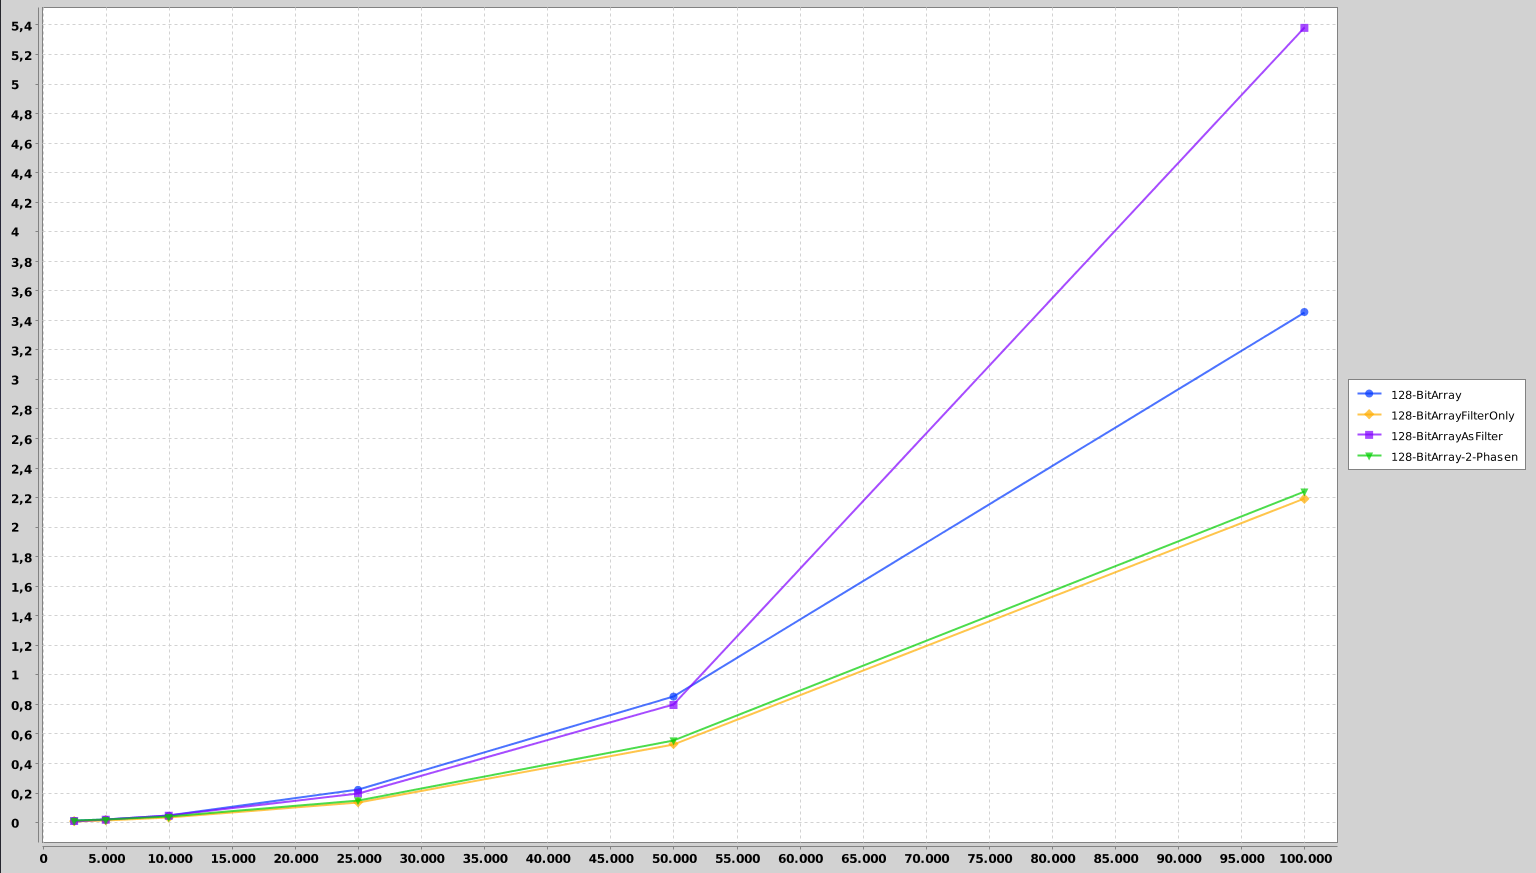
\includegraphics[width=1.07\textwidth, height=1.02\textheight]{Bilder/final_comparison_bit_array_approaches__threshold_0_7_trigram_one_fuzzy_date.png}

	\begin{tikzpicture}[overlay]
		\node at (3.65, 7)
		{
			\begin{footnotesize}
			\begin{varwidth}{0.6\textwidth}
			\textbf{Ausführungszeit in Minuten}
			\begin{itemize}
				\item für unterschiedlich große Datensätze
				\item Parameter
				\begin{itemize}
					\item Trigramme
					\item Threshold: $0.7$
					\item Datumsunschärfe: $1$
				\end{itemize}
				\item Testsystem
				\begin{itemize}
					\item CPU: 8 Kerne (HT) @ 3.4 GHz
					\item RAM: 16 GB
				\end{itemize}
			\end{itemize}
			\end{varwidth}
			\end{footnotesize}
		};
	\end{tikzpicture}
\end{frame}
